\documentclass[journal]{IEEEtran}

\usepackage{amsmath}
\usepackage{graphicx}
\usepackage{algorithm}
\usepackage{algorithmic}
\usepackage[colorlinks=true,allcolors=blue]{hyperref}

\graphicspath{{./figures/}}

\begin{document}

\title{Title of Your Paper}
\author{Author Name, Member, IEEE\thanks{Author affiliation and thanks to funding agencies.}}
\markboth{IEEE Journal Name}{Shell \MakeLowercase{\textit{et al.}}: Title of Paper}
\IEEEtitleabstractindextext{
	\begin{abstract}
		Abstract goes here. The abstract should be a brief summary of the paper, usually 150-250 words. It should state the problem, the methods used, the main results, and conclusions. Do not reference figures, tables, or equations in the abstract.
	\end{abstract}
	\begin{IEEEkeywords}
		keyword1, keyword2, keyword3, keyword4
	\end{IEEEkeywords}
}

\maketitle

\IEEEpeerreviewmaketitle

\section{Introduction}

Vector field analysis is a cornerstone of scientific visualization, providing critical insights into systems that involve particle interactions such as aerodynamics and fluid dynamic modeling, and areas that exhibit consistent forces such as gravitational modeling and magnetic fields.

These fields consist of a grid of discretely spaced points that are each assigned a vector.
This vector serves to store the strength and direction of motion around that point at a given instance.

To be able to effectively understand and analyze these fields, researchers rely on various models of these fields to identify key attributes such as vorticity, divergence, critical points, and flux.


\subsection{Streamline Analysis}

A streamline represents the path that an object would take if it moved through a static vector field. The path is traced by starting from a given vector and always proceeding in the direction of the current vector iteratively.
By connecting these directions throughout the field, streamlines illustrate how a substance or particle would flow at a particular instant.
This approach provides valuable insight into the topology of a given vector field.
This allows researchers to easily identify the overarching flow of a field, its sources and sinks, and other points of criticality.

Formally, a streamline is a curve that follows the direction of the vector field at every point, representing the path an object would take if it moved through the field at a given instant. For a steady vector field $\mathbf{v}(\mathbf{x})$, a streamline $\mathbf{x}(s)$ is defined by the differential equation:
\begin{equation}
	\frac{d\mathbf{x}}{ds} = \mathbf{v}(\mathbf{x}(s))
\end{equation}
where $s$ is a parameter along the curve.

These differ from pathlines, which seek to track a particle's progress over time.
In comparison, streamlines allow for a more comprehensive snapshot of entire vector fields at a static level; they can also be used to show how a given field changes over time, which is highly relevant to disciplines like magnetism.
This broader reach leads to a far higher complexity for streamline tracing in comparison to pathlines.


\begin{figure}[htbp]
	\centering
	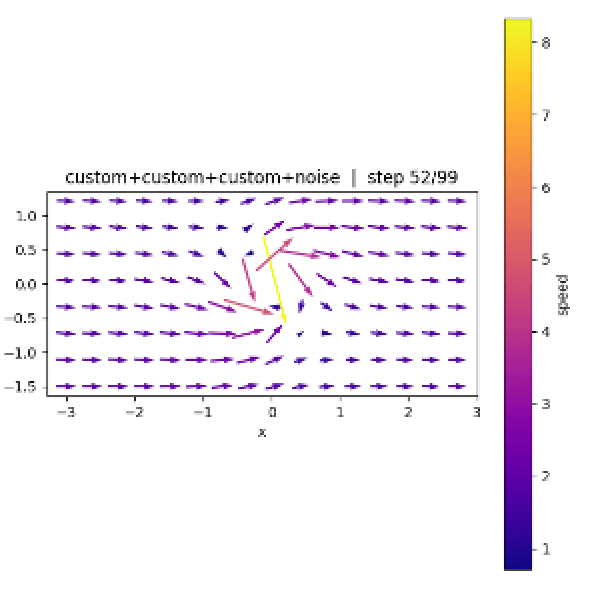
\includegraphics[width=0.8\linewidth]{media/vector-field.png}
	\caption{A discrete vector field grid representing force and direction at each point.}
	\label{fig:vector_field_grid}
\end{figure}

\begin{figure}[htbp]
	\centering
	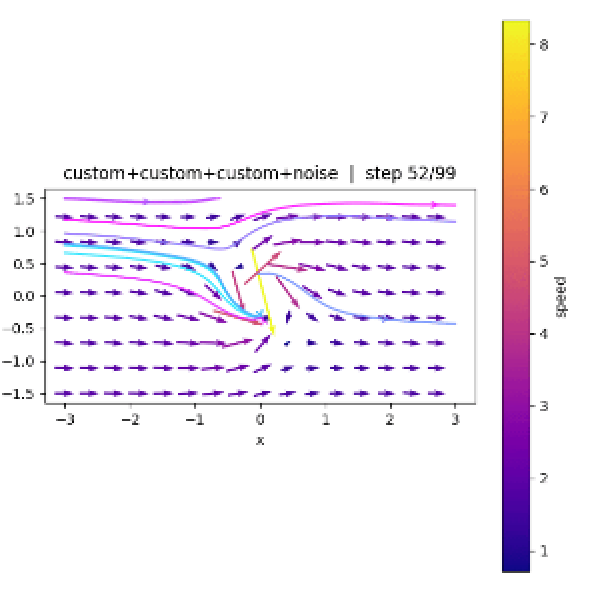
\includegraphics[width=0.8\linewidth]{media/vector-streams.png}
	\caption{A vector field grid with high-velocity streamlines highlighted to illustrate flow patterns.}
	\label{fig:vector_streams_highlighted}
\end{figure}


\subsection{Computational Challenges}

Despite their utility, streamline visualization faces significant computational overhead.

When analyzing large-scale datasets, such as those generated by high-fidelity simulations or astrophysical models, the computational cost of seeding and tracing thousands of streamlines becomes a bottleneck.

A major challenge arises from the irregular memory access patterns inherent in following a path through a grid.
Modern systems utilize caching to help ease the computational slowdown inherent to high I/O operations.
As streamlines are traced, vector points frequently point to subsequent vectors that fall outside of contiguous memory.
This leads to inefficient use of the cache and increased memory latency, which can significantly degrade performance on modern cache-hierarchical architectures.

The joining process of streamlines themselves also introduces challenges as it requires a store of information for each streamline that must be communicated globally to ensure that streamlines are treated as a continuous series.


Additionally, parallel implementations rely heavily on partitioning the dataset into smaller subdomains that can be processed independently.
Due to the inherent out-of-bounds access of vectors, parallel processes are forced to communicate across processes.
This introduces significant communication overhead.
This is especially apparent in GPU-accelerated and distributed implementations where data must be communicated and synchronized between processing units that don't have direct access to the isolated memory of other processes.

Together, these factors make efficient and scalable streamline computation a challenging problem in high-performance vector field analysis.


\subsection{Contributions}

This paper presents a research tool developed in C++17 for the accelerated analysis of 2D vector fields.

We address the computational bottleneck of streamline tracing by implementing and evaluating several parallel computing strategies.

Our primary contributions include:
\begin{itemize}
	\item A modular simulator for generating procedural vector fields (vortices, noise, and custom expressions) stored in HDF5 format.
	\item A suite of parallel analyzer implementations, ranging from shared-memory models (Pthreads, OpenMP) to distributed-memory (OpenMPI) and massively parallel GPU acceleration (CUDA).
	\item A comparative performance study demonstrating the scalability and speedup of these implementations across various field resolutions and streamline densities.
\end{itemize}

\section{Background}

This section should provide the necessary theoretical background and literature review. It should establish what is known about the topic and identify gaps that the current work addresses.

Key elements:
\begin{itemize}
	\item Review relevant prior work and literature
	\item Explain theoretical foundations
	\item Describe any existing methods or tools relevant to the work
	\item Identify gaps in existing research
\end{itemize}
\section{Methodology}

\subsection{Core Components}

\subsubsection{Vector Representation}
At the most fundamental level, the system utilizes a \texttt{Vec2} class to represent 2D vectors.
This class encapsulates two floating-point components, $x$ and $y$, and essential mathematical operations:
\begin{itemize}
	\item \textbf{Vector Arithmetic:} Standard operations for vector addition and scalar multiplication.
	\item \textbf{Normalization:} Methods to calculate the magnitude and derive unit vectors to allow for easy directional comparison.
\end{itemize}

\subsubsection{Field Representation}
Vector fields are represented as discretely spaced vectors stored within a grid structure.

The primary data structures are:
\begin{itemize}
	\item \texttt{FieldSlice}: A 2D grid of discretely spaced vectors.
	\item \texttt{FieldTimeSeries}: A collection of field slices associated with physical-space bounds ($x_{\text{min}}, x_{\text{max}}, y_{\text{min}}, y_{\text{max}}$).
	\item \texttt{FieldGrid}: Serves as the high-level manager for a single time-step's vector field, handling all the necessary calculations for streamline computations.
\end{itemize}

The \texttt{FieldReader} component handles the deserialization of these fields from HDF5 files using the HighFive library.
It extracts \texttt{vx} and \texttt{vy} datasets into the internal grid representation, ensuring that physical dimensions and time-series data are correctly mapped to the discrete grid indices.

\subsubsection{Grid Management and Streamline Tracing}

Each \texttt{Streamline} object stores an ordered list of grid coordinates (\texttt{row, col}) that constitutes a path.
This decouples the mathematical vector data from the state of the streamline tracing algorithm by maintaining a corresponding grid of \texttt{Streamline} pointers.
This abstraction allows the tracing logic to handle merging and path extension while keeping the underlying vector field read-only, which is critical for thread safety in parallel implementations.

\subsection{Streamline Tracing Algorithm}

The core logic for analyzing vector fields involves a discretized streamline tracing algorithm that maps continuous vector directions onto the underlying computational grid.
To manage the connectivity and merging of these paths efficiently, the system employs a Disjoint Set Union (DSU) or Union-Find algorithm.


\subsubsection{Discretized Subsequent Vector Calculation}
For each cell $(i, j)$, the algorithm computes the target subsequent vector by first determining the physical spacing between grid cells based on the field boundaries and grid dimensions.
It then advances the cell's physical position by the vector's $(x, y)$ components and converting back to grid indices using its knowledge of grid spacing.

\subsubsection{Connectivity Discovery via Union-Find to allow for Path Compression}
Using grid indices allows for the vector field grid to operate as a collection of disjoint sets where each disjoint set is a streamline.
The algorithm treats each grid cell as an element in a disjoint-set structure.
Connectivity is established by performing a \texttt{unite} operation between each cell and its calculated downstream subsequent vector.

The \texttt{unite} operation serves as the primary mechanism for establishing connectivity between grid cells.
In parallel contexts, this is performed using atomic synchronization primitives (e.g. barrier) to ensure that multiple threads can safely update the shared set structure without requiring heavy-weight locks.
To maintain high performance as the grid size increases, the algorithm employs path halving during the root discovery process, which incrementally flattens the tree structure and ensures that subsequent connectivity checks remain efficient.
This happens iteratively until it's subsection remains stable across passes.


This approach offers several advantages:
\begin{itemize}
	\item \textbf{Efficient Merging:} Streamlines that converge into the same cell are naturally merged into the same set, representing a single flow component.
	\item \textbf{Path Compression:} The \texttt{findRoot} operation, combined with path compression or halving, ensures that determining the component ownership of any cell is nearly constant time ($O(\alpha(n))$).
\end{itemize}

After all cells have been processed, the resulting disjoint sets represent the unique streamlines within the field.
Boundary effects and terminal points are handled naturally: if a vector points back to its own cell (after clamping), it remains its own root.

\subsection{Serial CPU Implementation}
The baseline implementation, \texttt{sequential CPU}, serves as a reference for both correctness and performance metrics.
It is implemented using modern C++17 standards and processes the vector field grid in a single pass using nested loops to iterate through rows and columns to identify it's subsequent vector.
Then each cell invokes the \texttt{traceStreamlineStep} method, which takes the original and subsequent vector and adds the subsequent vector to the streamline of the original.

\subsection{Shared-Memory Parallelism CPU Implementation}
To leverage multi-core architectures, we developed parallel implementations using POSIX Threads and OpenMP.
A significant challenge in parallelizing the streamline tracing algorithm is the stateful nature of the Union-Find structure; multiple threads performing \texttt{unite} operations could result in race conditions.
To address this, both shared-memory implementations employ a multi-pass strategy:
\begin{enumerate}
	\item \textbf{Parallel Subsequent Vector Precomputation:} The algorithm first calculates the destination subsequent vector for every cell in the grid.
	      Since this step only reads from the vector field and writes to an intermediate buffer, it is perfectly parallelizable.
	\item \textbf{Parallel Root Discovery:} After the sequential pass, the \texttt{findRoot} operation is performed in parallel for all cells to determine their final component assignments. \end{enumerate}

\subsubsection{POSIX Threads (Pthreads)}
The grid is partitioned into chunks where each thread is assigned a contiguous range of rows.
This minimizes the overhead of thread management while ensuring that each thread operates on a disjoint memory region in the subsequent vector buffer.
The implementation explicitly manages thread creation and joining, handling potential errors and ensuring that all threads terminate before proceeding to the sequential pass.

\subsubsection{OpenMP}
This works identically to the POSIX threads implementations with one modification.
We employ \texttt{\#pragma omp parallel for} directive with a \texttt{collapse(2)} clause to allow for easy segmentation and load balancing across our nested loops. T

\subsection{Massively Parallel GPU Acceleration with CUDA}
The CUDA implementation offloads the computationally intensive tasks of subsequent vector calculation and component discovery to the GPU, leveraging its high throughput to handle millions of cells simultaneously.
While it shares the multi-pass architecture of the parallel CPU implementations, it extends the parallelism to the connectivity analysis through the use of device-side synchronization primitives.

\begin{enumerate}
	\item \textbf{Parallel Subsequent Vector Precomputation:} A CUDA kernel assigns one thread to each grid cell to calculate its downstream subsequent vector.
	\item \textbf{Parallel Union-Find:} Unlike the shared-memory CPU versions which rely on a sequential merging pass, the CUDA implementation resolves streamline connectivity on the device using a parallel Union-Find algorithm. It employs \texttt{atomicCAS} (Compare-And-Swap) to ensure thread-safe updates to the disjoint-set.
	\item \textbf{Path Compression and Labeling:} A final kernel performs path compression, ensuring every cell points directly to its component root.
\end{enumerate}


\subsection{Distributed-Memory CPU Implementation}

The distributed-memory implementation using MPI introduces a significant challenge not present in the shared-memory implementations: processes do not share an address space, so the sequential Union-Find pass cannot operate globally across all ranks.
To address this, each rank is assigned a contiguous range of rows and independently computes and merges the downstream subsequent vectors for its assigned cells.
This correctly resolves all connections whose source cell falls within the rank's row range, but connections that cross rank boundaries are only partially recorded --- the source rank knows about the connection, but the destination rank does not.
We resolve these cross-boundary connections through an iterative \texttt{MPI\_Allreduce} loop, where each round broadcasts the current root of every cell across all ranks and takes the global minimum.
Any rank that observes a globally lower root for a cell than its own merges those two components locally via the \texttt{unite} operation, propagating that connectivity inward.
Each round resolves connections one rank boundary further, so at most $p$ rounds are needed for a field partitioned across $p$ ranks, with an early-exit condition terminating the loop as soon as no rank reports any changes.
Once all ranks have converged to a consistent global state, path reconstruction proceeds identically to the shared-memory implementations, with each rank building paths for its assigned cell range and the results gathered to rank 0.

\subsection{Distributed-Memory GPU Implementation (Hybrid)}

\subsection{Experimental Design}
This section outlines the setup and procedures for the scaling studies and performance evaluations conducted across different architectures.

\section{Results}

This section should present the findings of the research in a clear and logical manner. Use figures, tables, and graphs to illustrate the results effectively.

Guidelines:
\begin{itemize}
	\item Present results objectively without interpretation
	\item Use figures and tables with descriptive captions
	\item Reference all figures and tables in the text
	\item Include statistical analysis if applicable
	\item Compare results with existing methods when appropriate
\end{itemize}
\section{Conclusion}

The conclusion should summarize the main contributions, restate key findings, and discuss limitations and future work. It should not introduce new information but should provide a clear closure to the paper.

Key elements:
\begin{itemize}
	\item Summarize main contributions
	\item Highlight key results
	\item Discuss limitations of the work
	\item Suggest directions for future research
\end{itemize}
\section*{Acknowledgments}

We would like to thank the Center for High Performance Computing (CHPC) at the University of Utah for providing the computational resources and technical support that made this research possible.

\input{sections/references}

% Add a citation to generate bibliography entries
See \cite{ref1} for more information.

\end{document}


